\chapter{Java Grundlagen}
\renewcommand{\chaptertitle}{Java Grundlagen}

\lehead[]{\normalfont\sffamily\hspace*{-2.00cm}\textcolor{white}{\colorbox{lightblue}{\makebox[1.60cm][r]{\thechapter}}}\hspace{0.17cm}\textcolor{lightblue}{\chaptertitle}}
\rohead[]{\textcolor{lightblue}{\chaptertitle}\normalfont\sffamily\hspace*{0.17cm}\textcolor{white}{\colorbox{lightblue}{\makebox[1.60cm][l]{\thechapter}}}\hspace{-2.00cm}}
%\chead[]{}
\rehead[]{\textcolor{lightblue}{AvHG, Inf, My}}
\lohead[]{\textcolor{lightblue}{AvHG, Inf, My}}

\lstset{style=myJava}


\section{Wichtige Regeln}

\begin{compactitem}
\item Es wird zwischen Groß- und Kleinschreibung unterschieden!

\item Alle einzelnen Anweisungen müssen mit einem Semikolon (\lstinline|;|) beendet werden!

\item Mehrere Anweisungen können zu einem Anweisungsblock zusammengefasst
werden. Der Beginn eines Anweisungsblocks wird durch \lstinline|{| und das Ende
durch \lstinline|}| gekennzeichnet.

\item Prozeduren (tun etwas, liefern aber kein Ergebnis) und Funktionen (tun
etwas und geben ein Ergebnis als Rückgabewert zurück) werden in Java als
\emph{Methoden} bezeichnet. Methoden erkennt man immer an den runden Klammern
nach dem Namen. In diesen Klammern steht entweder nichts oder die Parameter, die
von der Methode verarbeitet werden.

Beispiele: \lstinline|close()|, \lstinline|compare(a, b)|

\item In Java ist es üblich, die Namen von Variablen und Methoden mit einem
kleinen Anfangsbuchstaben zu beginnen (auch wenn der Deutschlehrer das nicht
gut findet -- der sieht euren Code nicht!).

Beispiele: \lstinline|auto|, \lstinline|zeichneAuto()|

\item In Java ist jedes Programm eine \emph{Klasse}. Was das genau bedeutet,
werden wir uns später ansehen. Alle Variablen und Methoden müssen innerhalb der
geschweiften Klammern der Klasse stehen. Die Datei muss immer genauso
heißen wie die Klasse (mit der Dateiendung \texttt{.java}). Namen von Klassen
beginnen üblicherweise mit einem Großbuchstaben, z.\,B.\ \myClass{Auto},
\myClass{MeinProgramm}.
\end{compactitem}


\section{Variablen}

\subsection{Deklaration und Initialisierung}

Die \emph{Deklaration} (Vereinbarung) einer Variablen hat die Form:

\lstinline|Typname Variablenname;|

Beispiel:

\begin{lstlisting}
int i, j;
double zahl;
\end{lstlisting}

Bei der Deklaration darf die Variable auch gleichzeitig \emph{initialisiert}
werden. Das bedeutet, dass sie einen Anfangswert erhält. Beispiel:

\begin{lstlisting}
int i = 45, j = 3;
double zahl = 0.0;
\end{lstlisting}


\subsection{Lebensdauer (Gültigkeitsbereich)}

Die Lebensdauer einer lokalen Variablen, die innerhalb einer Methode deklariert
wird, erstreckt sich von der Stelle ihrer Deklaration bis zum Ende der Methode.
Falls eine Variable innerhalb eines geklammerten Blocks deklariert wird, lebt
die Variable nur bis zum Ende dieses Blocks.

Variablen, die außerhalb einer Methode direkt in der Klasse stehen (sogenannte
\emph{Attribute} bzw.\ Instanzvariablen), gehören zur gesamten Klasse und sind
in allen ihren Methoden sichtbar.


\subsection{Konstanten}

Einer Variable, deren Wert nicht verändert werden soll, wird das Schlüsselwort
\lstinline|final| vorangestellt. Damit wird die Variable zu einer
\emph{Konstanten}. Die Namen von Konstanten werden üblicherweise komplett groß
geschrieben. Beispiel:

\begin{lstlisting}
final float PI = 3.14f;
final String NAME = "Otto Mustermann";
\end{lstlisting}


\section{Kommentare}

\begin{lstlisting}
int i, j; æ// Kommentar bis zum Zeilenende

/* Kommentar über
 * mehrere Zeilen
 */æ
\end{lstlisting}


\section{Namenskonventionen}

Zur besseren Lesbarkeit des Codes gibt es folgende Konventionen:

\begin{tabular}{|l|l|l|l|}\hline
\textbf{Art} & \textbf{Namensgebung} & \textbf{Schreibweise} & \textbf{Beispiel}
\\ \hline
Klasse & Substantiv (Einzahl) & CamelCase mit großem Anfangsbuchstaben &
{\lstinline|String|}, {\lstinline|Auto|} \\ \hline
Variable, Objekt & Substantiv & camelCase mit
kleinem Anfangsbuchstaben & {\lstinline|meinAuto|} 
\\ \hline
Methode & Verb & camelCase mit kleinem
Anfangsbuchstaben & {\lstinline|zeichneAuto()|}
\\ \hline
Konstante & Substantiv & komplett mit Großbuchstaben &
{\lstinline|WIDTH|} 
\\
&& verbunden mit Unterstrichen &  {\lstinline|MIN_HEIGHT|}
\\ \hline
\end{tabular}

\medskip
Alle Namen müssen immer mit einem Buchstaben (oder Unterstrich/Dollarzeichen,
was aber unüblich ist) beginnen und dürfen keine Leerzeichen enthalten. 

Außerdem gilt als Grundregel: Bezeichner sollten möglichst kurz und \glqq
sprechend\grqq\ (selbsterklärend) sein. Ausgenommen von dieser Regel sind
Variablen, die nur kurzzeitig (etwa als Zähler innerhalb einer Schleife) benutzt
werden. Solche \glqq Wegwerfvariablen\grqq\ werden oft wie folgt benannt:

\lstinline|i|, \lstinline|j|, \lstinline|k|, \lstinline|m| und \lstinline|n|
für Ganzzahl-, \lstinline|x|, \lstinline|y| und \lstinline|z| für
Fließkomma- und schließlich \lstinline|c|, \lstinline|d| und
\lstinline|e| für Character-Variablen.

Siehe auch
\url{http://www.oracle.com/technetwork/java/codeconventions-135099.html}


\section{Datentypen}

Folgende Datentypen stehen zur Verfügung:

\begin{savenotes}
\begin{tabularx}{\textwidth}{|l|X|c|l|l|}\hline
\textbf{Datentyp} & \textbf{Bedeutung} & \textbf{Bytes} &
\textbf{Wertebereich} & \textbf{Standardwert}
\\ \hline
\texttt{boolean} & Wahrheitswerte & 1 & \texttt{true},
\texttt{false} & \texttt{false}
\\ \hline
\texttt{char} & Zeichen (Buchstaben) & 2 & Alle Unicode-Zeichen &
\texttt{\textbackslash u0000}
\\
&&(Fußnote\footnote{Einige seltene Unicode-Zeichen werden als eine Folge von
zwei \texttt{char}-Werten verpackt.\\ Siehe
\url{http://docs.oracle.com/javase/tutorial/i18n/text/unicode.html}})&&
\\
\hline \texttt{byte} & sehr kleine ganze Zahlen & 1 & $-128 \dots 127$ & \texttt{0}
\\ \hline
\texttt{short} & kleine ganze Zahlen & 2 & $-2^{15} \dots 2^{15}-1$
($-32.768 \dots 32.767$) & \texttt{0} \\ \hline
\texttt{int} & ganze Zahlen & 4 & $-2^{31} \dots 2^{31}-1$ & \texttt{0}
\\ \hline 
\texttt{long} & große ganze Zahlen & 8 & $-2^{63} \dots 2^{63}-1$ & \texttt{0}
\\ \hline
\texttt{float} & kleine Fließkommazahlen & 4 & $\pm 3{,}40282347 \cdot
10^{38}$ & \texttt{0.0f} \\ 
&&& (Fußnote\footnote{Tatsächlich ist der Wertebereich von \texttt{float} und
\texttt{double} im Negativen sogar minimal größer als im Positiven.\\ Siehe
\url{http://de.wikibooks.org/wiki/Java_Standard:_Primitive_Datentypen}})&
\\
\hline \texttt{double} & große Fließkommazahlen & 8 & $\pm 1{,}79769313486231570
\cdot 10^{308}$ & \texttt{0.0}
\\ \hline
\texttt{String} & Zeichenketten & -- & beliebig lange Texte & \texttt{null}
\\ \hline
\end{tabularx}
\end{savenotes}

\medskip
Neben den primitiven Standard-Datentypen kann man sich eigene Datentypen
definieren, indem man eine eigene Klasse schreibt. Der Typ \myClass{String} ist
eine bereits vordefinierte Klasse aus dem Package \myPackage{java.lang}.


\section{Typkonvertierungen}

Zwischen den primitiven Datentypen besteht die folgende Beziehung:

\begin{center}
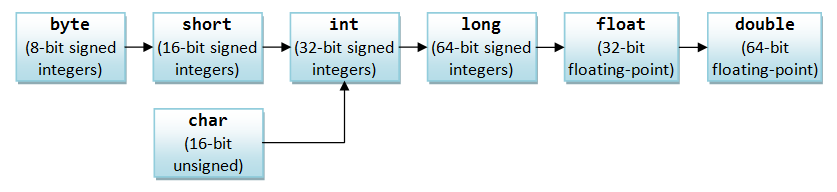
\includegraphics[width=0.9\textwidth]{./inf/SEKII/04_Java_Grundlagen/JavaBasics_ImplicitTypeCastingPrimitives.png}
% Quelle: http://ntu.edu.sg/home/ehchua/programming/java/J2_Basics.html
% erlaubnis zur verwendung per e-mail von ehchua@ntu.edu.sg vom 5.8.13:
% --- snip -----
% You can use for teaching in public schools, but not for commercial purposes.
% Hock Chuan
% --- snap -----
\end{center}

Die Konvertierung eines „kleineren“ in einen „größeren“ Datentyp (also von links
nach rechts im Schaubild) führt das System automatisch durch. Eine Konvertierung
in umgekehrter Richtung kann einen Datenverlust bedeuten und wird deshalb nur
auf explizite Anweisung des Programmierers vorgenommen. Beispiel:

\begin{lstlisting}
int i = 56;
double d = 24.5;
double d2 = i;      æ// geht automatisch
æint i2 = (int) d;   æ// explizite Typkonvertierung, vom Programmierer erzwungen (= 24)
æchar c = (char) i;  æ// explizite Typkonvertierung (Unicode-Zeichen 56 = '8')
\end{lstlisting}

Das Schema einer expliziten Typkonvertierung (sogenanntes \emph{Type Casting}) lautet:

\verb|Variable_vom_Typ1 = (Typ1) Variable_vom_Typ2;|

Andere Konvertierungen (z.\,B.\ zwischen \lstinline|int| und \lstinline|String|)
können nur mithilfe spezieller Methoden durchgeführt werden. Zahlenvariablen
werden jedoch automatisch in einen \lstinline|String| umgewandelt, wenn man sie
mit einem \lstinline|+|-Zeichen an einen \lstinline|String| anhängt. Beispiel:

\begin{lstlisting}
String text = "Der Inhalt von i ist: " + i;
\end{lstlisting}


\section{Literale}

\begin{description}
\item{\textbf{Ganzzahlige Zahlenwerte}} (z.\,B.\ \lstinline|304|) sind
grundsätzlich vom Typ \lstinline|int|. Nur wenn das Suffix \lstinline|l| oder \lstinline|L| hinten
angehängt wird (z.\,B.\ \lstinline|304L|), sind sie vom Typ \lstinline|long|.

\item{\textbf{Zahlenwerte von Fließkommazahlen}} enthalten im Gegensatz zu
ganzen Zahlen einen Punkt zur Trennung der Nachkommastellen (z.\,B.\ ist \lstinline|0| eine ganze Zahl,
aber \lstinline|0.0| ist eine Fließkommazahl). Standardmäßig sind
Fließkommazahlen vom Typ \lstinline|double|. Wenn man eine Fließkommazahl vom
Typ \lstinline|float| haben möchte, muss man das Suffix \lstinline|f| oder
\lstinline|F| an die Zahl anhängen (z.\,B.\ \lstinline|0.0F|).

Für Fließkommazahlen sind einige symbolische Zahlenwerte verfügbar:

\begin{tabular}{|l|l|}\hline
\textbf{Name} & \textbf{Bedeutung} \\ \hline
{\lstinline|MAX_VALUE|} & Größter darstellbarer positiver Wert \\ \hline
{\lstinline|MIN_VALUE|} & Kleinster darstellbarer positiver Wert \\ \hline
{\lstinline|NaN|} & Not-A-Number (ungültiges Rechenergebnis, z.\,B.\ $0{,}0 / 0{,}0$) \\ \hline
{\lstinline|NEGATIVE_INFINITY|} & Negativ unendlich \\ \hline
{\lstinline|POSITIVE_INFINITY|} & Positiv unendlich \\ \hline
\end{tabular}

\item{\textbf{Einzelne Zeichen (\lstinline|char|)}} werden grundsätzlich in einfache
Hochkommata gesetzt (z.\,B.\ \lstinline|'a'|).

\item{\textbf{Zeichenketten (\lstinline|String|)}} werden mit doppelten
Hochkommata geschrieben. Zur Darstellung von Sonderzeichen gibt es eine Reihe
von Standard-Escape-Sequenzen:

\begin{tabular}{|l|l|}\hline
\textbf{Zeichen} & \textbf{Bedeutung} \\ \hline
{\lstinline|\b|} & Rückschritt (Backspace) \\ \hline
{\lstinline|\t|} & Horizontaler Tabulator \\ \hline
{\lstinline|\n|} & Zeilenschaltung (Newline) \\ \hline
{\lstinline|\f|} & Seitenumbruch (Formfeed) \\ \hline
{\lstinline|\r|} & Wagenrücklauf (Carriage return) \\ \hline
{\lstinline|\"|} & Doppeltes Anführungszeichen \\ \hline
{\lstinline|\'|} & Einfaches Anführungszeichen \\ \hline
{\lstinline|\\|} & Backslash \\ \hline
{\lstinline|\nnn|} & Oktalzahl \texttt{nnn} (kann auch kürzer als 3 Zeichen sein, darf
nicht größer als oktal 377 sein) \\ \hline
{\lstinline|\uxxxx|} & Unicode-Escape-Sequenz. \texttt{xxxx} steht für eine Folge von 4
hexadezimalen Ziffern.\\
& Z.\,B.\ ist {\lstinline|\u0020|} die Hexadezimaldarstellung des Leerzeichens.
\\ \hline
\end{tabular}

Beispiele:

\begin{lstlisting}
char c = 'a', b = '\t';
String text = "Guten Tag.\nWie geht es dir?";
\end{lstlisting}
\end{description}


\section{Operatoren}

\subsection{Arithmetische Operatoren}

\begin{tabularx}{\textwidth}{|c|l|X|}\hline
\textbf{Operator} & \textbf{Bezeichnung} & \textbf{Bedeutung}
\\ \hline
\texttt{+} & Addition & \texttt{a + b} ergibt die Summe von
\texttt{a} und \texttt{b}.
\\ \hline
\texttt{-} & Subtraktion & \texttt{a - b} ergibt die Differenz von
\texttt{a} und \texttt{b}.
\\ \hline
\texttt{*} & Multiplikation & \texttt{a * b} ergibt das Produkt
von \texttt{a} und \texttt{b}.
\\ \hline
\texttt{/} & Division & \texttt{a / b} ergibt den Quotienten
von \texttt{a} und \texttt{b} (Achtung: bei zwei Ganzzahlen Ganzzahldivision!).
\\ \hline
\texttt{\%} & Modulo (Restwert) & \texttt{a \% b} ergibt den Rest der
ganzzahligen Division von \texttt{a} und \texttt{b}. Lässt sich in Java auch auf Fließkommazahlen anwenden.
\\ \hline
\texttt{++} & Präinkrement & \texttt{x = ++a;} erhöht \texttt{a}
um \texttt{1} und schreibt das Ergebnis (\texttt{a+1}) in
\texttt{x}.
\\ \hline
\texttt{++} & Postinkrement & \texttt{x = a++;} schreibt
\texttt{a} in \texttt{x} und erhöht \texttt{a} anschließend um
\texttt{1}.
\\ \hline
\texttt{--} & Prädekrement & \texttt{x = --a;} verringert
\texttt{a} um \texttt{1} und schreibt das Ergebnis (\texttt{a-1})
in \texttt{x}.
\\ \hline
\texttt{--} & Postdekrement & \texttt{x = a--;} schreibt
\texttt{a} in \texttt{x} und verringert \texttt{a} anschließend
um \texttt{1}.
\\ \hline
\end{tabularx}


\subsection{Vergleichs-Operatoren}

\begin{tabularx}{\textwidth}{|c|l|X|}\hline
\textbf{Operator} & \textbf{Bezeichnung} & \textbf{Bedeutung}
\\ \hline
\texttt{==} & gleich & \texttt{a == b} ergibt \texttt{true}, wenn
\texttt{a} gleich \texttt{b} ist. Sind \texttt{a} und
\texttt{b} Referenztypen, so ist der Rückgabewert \texttt{true}, wenn beide Werte auf dasselbe Objekt zeigen.
\\ \hline
\texttt{!=} & ungleich & \texttt{a != b} ergibt \texttt{true},
wenn \texttt{a} ungleich \texttt{b} ist. Sind \texttt{a} und
\texttt{b} Objekte, so ist der Rückgabewert
\texttt{true}, wenn beide Werte auf unterschiedliche Objekte zeigen.
\\ \hline
\texttt{<} & kleiner & \texttt{a < b} ergibt \texttt{true}, wenn
\texttt{a} kleiner \texttt{b} ist.
\\ \hline
\texttt{<=} & kleiner gleich & \texttt{a <= b} ergibt
\texttt{true}, wenn \texttt{a} kleiner oder gleich \texttt{b}
ist.
\\ \hline
\texttt{>} & größer & \texttt{a > b} ergibt \texttt{true}, wenn
\texttt{a} größer \texttt{b} ist.
\\ \hline
\texttt{>=} & größer gleich & \texttt{a >= b} ergibt
\texttt{true}, wenn \texttt{a} größer oder gleich \texttt{b}
ist.
\\ \hline
\end{tabularx}

\medskip
\noindent \textbf{Wichtiger Hinweis zu Strings:} Zeichenketten (\lstinline|String|)
sind Objekte! Um zu prüfen, ob zwei Strings denselben Text enthalten, benutzt
man daher \textbf{nicht} \lstinline|==|, sondern die Methode
\lstinline|text1.equals(text2)|.


\subsection{Logische Operatoren}

\begin{tabularx}{\textwidth}{|c|p{3.4cm}|X|}\hline
\textbf{Operator} & \textbf{Bezeichnung} & \textbf{Bedeutung}
\\ \hline
\texttt{!} & logisches NICHT & \texttt{!a} ergibt \texttt{false},
wenn \texttt{a} wahr ist, und \texttt{true}, wenn \texttt{a}
falsch ist.
\\ \hline
\texttt{\&\&} & UND mit Short-Circuit-Evaluation &
\texttt{a \&\& b} ergibt \texttt{true}, wenn sowohl \texttt{a} als
auch \texttt{b} wahr sind. Ist \texttt{a} bereits falsch, so wird
\texttt{false} zurückgegeben und \texttt{b} nicht mehr ausgewertet.
\\ \hline
\texttt{||} & ODER mit Short-Circuit-Evaluation &
\texttt{a || b} ergibt \texttt{true}, wenn mindestens einer der beiden
Ausdrücke \texttt{a} oder \texttt{b} wahr ist. Ist bereits
\texttt{a} wahr, so wird \texttt{true} zurückgegeben und
\texttt{b} nicht mehr ausgewertet.
\\ \hline
\texttt{\&} & UND ohne Short-Circuit-Evaluation &
\texttt{a \& b} ergibt \texttt{true}, wenn sowohl \texttt{a} als
auch \texttt{b} wahr sind. Beide Teilausdrücke werden ausgewertet.
\\ \hline
\texttt{|} & ODER ohne Short-Circuit-Evaluation &
\texttt{a | b} ergibt \texttt{true}, wenn mindestens einer der beiden
Ausdrücke \texttt{a} oder \texttt{b} wahr ist. Beide
Teilausdrücke werden ausgewertet.
\\ \hline
\texttt{\^{}} & Exklusiv-ODER & \texttt{a \^{} b} ergibt \texttt{true},
wenn beide Ausdrücke einen unterschiedlichen Wahrheitswert haben.
\\ \hline
\end{tabularx}


\subsection{Zuweisungsoperatoren}

\begin{tabularx}{\textwidth}{|c|l|X|}\hline
\textbf{Operator} & \textbf{Bezeichnung} & \textbf{Bedeutung}
\\ \hline
\texttt{=} & einfache Zuweisung & \texttt{a = b;} weist
\texttt{a} den Wert von \texttt{b} zu und liefert \texttt{b} als
Rückgabewert.
\\ \hline
\texttt{+=} & Additionszuweisung & \texttt{a += b;} ist eine Abkürzung
für \texttt{a = a + b;}.
\\ \hline
\texttt{-=} & Subtraktionszuweisung & \texttt{a -= b;} ist eine
Abkürzung für \texttt{a = a - b;}.
\\ \hline
\texttt{*=} & Multiplikationszuweisung & \texttt{a *= b;} ist
eine Abkürzung für \texttt{a = a * b;}.
\\ \hline
\texttt{/=} & Divisionszuweisung & \texttt{a /= b;} ist
eine Abkürzung für \texttt{a = a / b;}.
\\ \hline
\texttt{\%=} & Modulozuweisung & \texttt{a \%= b;} ist eine Abkürzung
für \texttt{a = a \% b;}.
\\ \hline
\end{tabularx}

\clearpage

\section{Kontrollstrukturen}

\subsection{Einfache Verzweigung}

\begin{lstlisting}
if (`\slshape{Bedingung}`) {
  `\slshape{Anweisungen}`;
}
else {
  `\slshape{Anweisungen}`;
}
\end{lstlisting}

Der \lstinline|else|-Teil kann auch entfallen. Die geschweiften Klammern dürfen
weggelassen werden, wenn es nur eine einzige Anweisungszeile gibt (aus Gründen
der Übersichtlichkeit und Fehlervermeidung empfiehlt es sich aber, sie immer zu
setzen).

\subsection{Mehrfach-Verzweigung}

\subsubsection{switch ohne Rückgabewert}

\begin{lstlisting}
switch (`\slshape{Ausdruck}`) {
  case `\slshape{Wert1}`, `\slshape{Wert2}` -> `\slshape{Anweisung}`;
  case `\slshape{Wert3}`, `\slshape{Wert4}`, `\slshape{Wert5}` -> {
    `\slshape{Anweisungsblock}`
  }
  ...
  default -> `\slshape{Anweisung}`;         æ// falls kein anderer Wert passt (optional)
æ}
\end{lstlisting}

Beispiel:

\begin{lstlisting}
switch (ampelfarbe) {
  case "rot", "gelb" -> warten();
  case "grün" -> gehen();
  default -> System.out.println("Das ist aber eine komische Ampel!");
}
\end{lstlisting}

\subsubsection{switch mit Rückgabewert}

\begin{lstlisting}
`\slshape{datentyp variable}` = switch (`\slshape{Ausdruck}`) {
  case `\slshape{Wert1}`, `\slshape{Wert2}` -> `\slshape{Rückgabewert1}`;
  case `\slshape{Wert3}`, `\slshape{Wert4}`, `\slshape{Wert5}` -> `\slshape{Rückgabewert2}`;
  ...
  default -> `\slshape{Default-Rückgabewert}`;
};
\end{lstlisting}

Beispiel:

\begin{lstlisting}
String alterskategorie = switch (alter) {
  case 0, 1, 2, 3, 4, 5, 6, 7, 8, 9, 10, 11, 12 -> "Kinder";
  case 13, 14, 15, 16, 17 -> "Jugendliche";
  default -> "Erwachsene";
};
\end{lstlisting}

\subsection{Schleifen}

\begin{compactenum}[a)]
\item \textbf{Kopfgesteuerte Schleife (\lstinline|while|):}
\begin{lstlisting}
while (`\slshape{Bedingung}`) {
  `\slshape{Anweisungen}`;
}
\end{lstlisting}

Beispiel:

\begin{lstlisting}
int zaehler = 0;
while (zaehler < 10) {
  System.out.println("Der Zähler hat den Wert: " + zaehler);
  zaehler++;     æ// Kurzform für: zaehler = zaehler + 1;
æ}
\end{lstlisting}

Die Anweisungen in den geschweiften Klammern werden ausgeführt, solange die
Bedingung \lstinline|true| ergibt.

\item \textbf{Fußgesteuerte Schleife (\lstinline|do-while|):}
\begin{lstlisting}
do {
  `\slshape{Anweisungen}`;
} while (`\slshape{Bedingung}`);
\end{lstlisting}

Die Anweisungen in den geschweiften Klammern werden ausgeführt, solange die
Bedingung \lstinline|true| ergibt (mindestens aber einmal).

\item \textbf{Zählschleife (\lstinline|for|):}
\begin{lstlisting}
for (`\slshape{Vorab}`; `\slshape{Bedingung}`; `\slshape{Wert-Verändern}`) {
  `\slshape{Anweisungen}`;
}
\end{lstlisting}

Der Teil \emph{Vorab} wird nur einmal ausgeführt, bevor die Schleife
betreten wird. Hier fügt man den Code zur Initialisierung der Zählvariable ein.
Die Schleife wird ausgeführt, solange die \emph{Bedingung} wahr ist. Nach
jedem Schleifendurchgang wird der Code \emph{Wert-Verändern} einmal
ausgeführt. Das obige Beispiel für die \lstinline|while|-Schleife kann man mit
der \lstinline|for|-Schleife folgendermaßen schreiben:

\begin{lstlisting}
for (int zaehler = 0; zaehler < 10; zaehler++) {
  System.out.println("Der Zähler hat den Wert: " + zaehler);
}
\end{lstlisting}
\end{compactenum}


\section{Methoden}

Aufgaben, die mehrere Anweisungen umfassen und die immer wieder -- auch an
verschiedenen Stellen des Programms -- ausgeführt werden sollen, kann man in
\emph{Methoden} \glqq verpacken\grqq :

Methoden müssen immer innerhalb einer Klasse stehen. Eine Methode hat
folgendes Schema:

\begin{lstlisting}
`\slshape{Sichtbarkeit Rückgabewert Name}`(`\slshape{Typ1 Parameter1}`, `\slshape{Typ2 Parameter2}`, ...) {
  `\slshape{Anweisungen}`;
  return `\slshape{Wert}`;         æ// Rückgabe eines berechneten Wertes. Kann entfallen.
æ}
\end{lstlisting}

Die \emph{Sichtbarkeit} regelt, wer das Recht hat, die Methode aufzurufen. Der
Wert \lstinline|public| gibt z.\,B.\ an, dass die Methode öffentlich ist und jeder
darauf zugreifen kann.

Der \emph{Rückgabewert} gibt an, welchen Typ die Werte haben, die die Methode
zurückliefert. Wenn die Methode keinen Wert zurückliefert, schreibt man
\lstinline|void|. Wenn die Methode einen Wert zurückgibt, gibt man an dieser
Stelle den Typ des Werts an.

Primitive Standard-Datentypen (\lstinline|int|, \lstinline|boolean|, usw.) werden
in Java als Werte-Parameter übergeben, d.\,h.\ es wird eine Kopie des Werts
übergeben. Objekt-Variablen sind dagegen Referenz-Parameter, d.\,h.\ es wird
eine Kopie der Speicheradresse des Objekts übergeben (Änderungen am Objekt
innerhalb der Methode wirken sich also auch außerhalb aus).

Beispiele:

\begin{lstlisting}
public void schreibeText() {
  System.out.println("Hallo");          æ// schreibt Text auf die Konsole
æ}

public int mult(int zahl1, int zahl2) {
  int ergebnis = zahl1 * zahl2;
  return ergebnis;
}
\end{lstlisting}

Der Aufruf der obigen Methoden von einer anderen Methode innerhalb derselben Klasse kann z.\,B.
folgendermaßen aussehen:

\begin{lstlisting}
schreibeText();                         æ// die Klammern dürfen nicht fehlen!
æint zahl = mult(5, 4);
\end{lstlisting}